\documentclass[a4paper]{article}
\usepackage[fontsize=12pt]{scrextend}



\usepackage{tikz}
\usetikzlibrary{positioning,arrows.meta,shapes.geometric}

% --- Настройка шрифтов и локализации для XeLaTeX ---
\usepackage{fontspec}
\usepackage{xunicode}
\usepackage{xltxtra}
\usepackage{polyglossia}
\setmainlanguage{russian}
\setotherlanguage{english}
\defaultfontfeatures{Ligatures=TeX}
\setmainfont{Times New Roman}
\newfontfamily\cyrillicfont{Times New Roman}
\setmonofont{Courier New}
\newfontfamily\cyrillicfonttt{Courier New}

% --- Параметры страницы по ГОСТ 7.32-2017 (левое 30 мм, правое 10 мм, верхнее и нижнее по 20 мм) ---
\usepackage[left=30mm, right=10mm, top=20mm, bottom=20mm]{geometry}

% --- Интервалы и абзацный отступ (1.25 см, 1.5 интервал) ---
\usepackage{indentfirst}
\setlength{\parindent}{1.25cm}
\usepackage{setspace}
\onehalfspacing

% --- Пакеты для таблиц, списков и графики ---
\usepackage{tabularx}
\usepackage{booktabs}
\usepackage{array}
\usepackage{enumitem}
\setlist{nosep, leftmargin=\parindent}
\usepackage{graphicx}

% --- Листинги кода с подсветкой синтаксиса ---
\usepackage{listings}
\usepackage{xcolor}

\lstset{
    basicstyle=\ttfamily\footnotesize,
    columns=flexible,
    keepspaces=true,
    breaklines=true,
    frame=single,
    tabsize=4,
    showstringspaces=false,
    keywordstyle=\bfseries\color{blue!70!black},
    commentstyle=\itshape\color{green!50!black},
    stringstyle=\color{red!60!black},
    numbers=none
}

% --- Оформление заголовков по ГОСТ 7.32-2017 ---
\usepackage{titlesec}
\titleformat{\section}[block]
  {\normalfont\bfseries\filright}
  {\hspace{1.25cm}\thesection\quad}
  {0pt}
  {\MakeUppercase}

\titleformat{\subsection}[block]
  {\normalfont\bfseries\filright}
  {\hspace{1.25cm}\thesubsection\quad}
  {0pt}
  {}

\titleformat{\subsubsection}[block]
  {\normalfont\bfseries\filright}
  {\hspace{1.25cm}\thesubsubsection\quad}
  {0pt}
  {}

\titlespacing*{\section}{0pt}{18pt}{12pt}
\titlespacing*{\subsection}{0pt}{12pt}{6pt}
\titlespacing*{\subsubsection}{0pt}{10pt}{4pt}

% Подписи к рисункам и таблицам по ГОСТ
\usepackage[tableposition=top,figureposition=bottom]{caption}
\DeclareCaptionLabelSeparator{emdash}{~---~}
\captionsetup[figure]{
  name={Рисунок},
  labelsep=emdash,
  font={normalsize},
  justification=centering,
  singlelinecheck=true
}
\captionsetup[table]{
  name={Таблица},
  labelsep=emdash,
  font={normalsize},
  justification=raggedright,
  singlelinecheck=false,
  margin=0pt
}

% --- Отточие в содержании ---
\usepackage{tocloft}
\renewcommand{\cftsecleader}{\cftdotfill{\cftdotsep}}
\renewcommand{\cfttoctitlefont}{\hfill\bfseries\MakeUppercase}
\renewcommand{\cftaftertoctitle}{\hfill}

\begin{document}

% =========================================================================
% ТИТУЛЬНЫЙ ЛИСТ
% =========================================================================
\begin{titlepage}
    \centering
    {\small МИНИСТЕРСТВО НАУКИ И ВЫСШЕГО ОБРАЗОВАНИЯ РОССИЙСКОЙ ФЕДЕРАЦИИ}\\
    {\scriptsize \textbf{ФЕДЕРАЛЬНОЕ ГОСУДАРСТВЕННОЕ АВТОНОМНОЕ ОБРАЗОВАТЕЛЬНОЕ УЧРЕЖДЕНИЕ ВЫСШЕГО ОБРАЗОВАНИЯ}}\\
    {\bfseries «НАЦИОНАЛЬНЫЙ ИССЛЕДОВАТЕЛЬСКИЙ УНИВЕРСИТЕТ ИТМО»}\\[0.8cm]

    \textbf{Факультет безопасности информационных технологий}\\[0.6cm]

    \textbf{Направление подготовки: 10.03.01 Информационная безопасность} \\
    \textbf{Образовательная программа: «Технологии защиты информации»} \\[0.6cm]

    \textbf{Дисциплина:} \\
    \textit{\textbf{«Технологии и методы программирования»}} \\ [1.5cm]

    {\bfseries ОТЧЕТ ПО ЛАБОРАТОРНОЙ РАБОТЕ №2}\\
    \textit{{\bfseries «Разработка программного обеспечения с механизмами контроля лимитов пробного использования (Trial-версия) и защитой от переустановки»}}\\[3.5cm]

    \begin{flushright}
        \textbf{Выполнил студент:} \\ [0.5em]
        Пахомов Владимир Юрьевич / \raisebox{-0.3\height}{
\includegraphics[width=1.3cm]{sign1.png}} \\
        {\scriptsize{\textit{ФИО \hspace{2cm} Подпись \hspace{0.3cm}}}} \\ [0.3cm]

        \textbf{Проверил:}\\ [0.5em]
        Ищенко Алексей Петрович / \underline{\hspace{2.5cm}} \\
        {\scriptsize{\textit{ФИО \hspace{2.5cm} Подпись \hspace{0.5cm}}}} \\ [1.5cm]

        {\scriptsize \underline{\hspace{4cm}}} \\
        {\scriptsize \textit{Отметка о выполнении}} \\
        {\scriptsize \underline{\hspace{4cm}}} \\
        {\scriptsize \textit{Дата}}
    \end{flushright}

    \vfill
    Санкт-Петербург\\
    2026
\end{titlepage}

% =========================================================================
% СОДЕРЖАНИЕ
% =========================================================================
\newpage
\pagestyle{plain}
\setcounter{page}{2}

\begin{center}
    {\bfseries \MakeUppercase{Содержание}}
\end{center}
\vspace{-0.5cm}
\tableofcontents

% =========================================================================
% ВВЕДЕНИЕ
% =========================================================================
\newpage
\begin{center}
    {\bfseries \MakeUppercase{Введение}}
\end{center}
\addcontentsline{toc}{section}{ВВЕДЕНИЕ}

\textbf{Цель работы}: приобретение практических навыков реализации прикладных механизмов защиты программных продуктов от несанкционированного тиражирования и неправомерного продления ознакомительного периода, разработка программного комплекса (инсталлятор, приложение, деинсталлятор) с комбинированным ограничением по времени и числу запусков, а также проведение анализа защищенности системы и способов ее обхода («взлома»).

\textbf{Постановка задачи}:
\begin{enumerate}
    \item Разработать программу, запрашивающую у пользователя фамилию, имя и отчество (ФИО) и сохраняющую их в файл профиля. При совпадении введенных данных с сохраненными ранее выводить соответствующее сообщение.
    \item Реализовать две версии программы (или одну совмещенную):
          \begin{itemize}
              \item \textit{Time-limited}: ограничение по времени жизненного цикла ознакомительного режима с момента первого старта (не более 3 минут).
              \item \textit{Start-limited}: жесткое ограничение по количеству запусков приложения (например 4-5 запусков);
          \end{itemize}
    \item При исчерпании любого из лимитов блокировать ввод данных и предлагать пользователю два действия: переход к приобретению полной лицензии либо запуск встроенного деинсталлятора.
    \item Разработать графический инсталлятор, регистрирующий ПО в среде пользователя.
    \item Обеспечить сохранение истории лицензирования: при повторной установке инсталлятор обязан детектировать факт прошлой инсталляции, информировать пользователя об израсходованном лимите и запрещать сброс счетчиков.
    \item Разработать деинсталлятор, корректно очищающий исполняемые бинарные файлы и ярлыки рабочего окружения, но сохраняющий скрытый маркер лицензирования.
\end{enumerate}

% =========================================================================
% 1. АРХИТЕКТУРА И АЛГОРИТМЫ СИСТЕМЫ ЗАЩИТЫ
% =========================================================================
\newpage
\section{Архитектура и алгоритмы системы защиты ПО}

\subsection{Общая структура программного комплекса}
Программный комплекс спроектирован по модульному принципу и ориентирован на исполнение в современных дистрибутивах Linux с поддержкой стандартов XDG Base Directory Specification и графического окружения KDE Plasma.

Комплекс включает три ключевых компонента:
\begin{enumerate}
    \item \textbf{Модуль установки (\texttt{installer.py})}: выполняет проверку предыдущих установок, развертывает файлы в системные пути пользователя, создает \texttt{.desktop}-файлы для интеграции в меню программ и на Рабочий стол, а также валидирует доверенные атрибуты запуска через подсистему GIO;
    \item \textbf{Основное приложение (\texttt{main.py})}: графическая утилита на базе Tkinter, реализующая логику проверки лицензионных ограничений, обработку ФИО и выполнение блокировки функционала;
    \item \textbf{Модуль деинсталляции (\texttt{uninstaller.py})}: осуществляет безопасное удаление исполняемых компонентов программы и интеграций с рабочим столом, сохраняя лицензионный артефакт в каталоге конфигураций пользователя.
\end{enumerate}


\subsection{Структура хранения лицензионных данных}
В соответствии со спецификацией XDG, конфигурационный каталог пользователя располагается по пути \texttt{\textasciitilde/.config/lab2/}. В нем создается структурированный текстовый файл \texttt{lab2.txt}. Структура файла описана в таблице~\ref{tab:conf_spec}.

\begin{table}[h!]
    \caption{Спецификация строк файла конфигурации и лицензии \texttt{lab2.txt}}
    \label{tab:conf_spec}
    \small
    \begin{tabularx}{\textwidth}{|c|l|p{4cm}|X|}
        \hline
        \textbf{№ строки} & \textbf{Поле}          & \textbf{Тип данных}      & \textbf{Назначение}                                    \\ \hline
        1                 & \texttt{name}          & Текстовая строка (UTF-8) & Хранение зарегистрированного ФИО пользователя          \\ \hline
        2                 & \texttt{launches}      & Целое неотрицательное    & Счетчик совершенных запусков приложения (Start-limit)  \\ \hline
        3                 & \texttt{first\_launch} & Строка ISO-8601 UTC      & Временная метка первого запуска программы (Time-limit) \\ \hline
    \end{tabularx}
\end{table}

\subsection{Алгоритм контроля ограничений}
Приложение сочетает в себе два независимых механизма контроля: по количеству запусков и по времени с момента первого сохранения ФИО.
При каждом старте выполняется проверка условий, и если хотя бы одно из них нарушено, интерфейс блокируется, предлагая пользователю деинсталлировать программу или связаться с поддержкой. Под запуском программы подразумевается сохранение ФИО в файл: именно тогда счетчик увеличивается на единицу, а временная метка фиксируется при первом сохранении.


% =========================================================================
% 2. РЕАЛИЗАЦИЯ ПРОГРАММНЫХ КОМПОНЕНТОВ
% =========================================================================
\newpage
\section{Реализация программных компонентов}

\subsection{Инсталлятор и обнаружение повторной установки}
Инсталлятор (\texttt{installer.py}) реализует полный цикл развертывания приложения без необходимости прав суперпользователя (\texttt{root}), используя домашний каталог пользователя согласно спецификациям freedesktop.org:
\begin{itemize}
    \item Исполняемые файлы копируются в директорию \texttt{\textasciitilde/.local/share/lab2/};
    \item Интеграция в системное меню приложений рабочего окружения выполняется путем генерации \texttt{.desktop} файла в \texttt{\textasciitilde/.local/share/applications/lab2.desktop};
    \item Автоматически определяется каталог Рабочего стола с запасными путями (\texttt{\textasciitilde/Desktop}, \texttt{\textasciitilde/Рабочий стол}) и создается ярлык запуска.
\end{itemize}

Перед началом копирования файлов процедура \texttt{check\_previous\_install()} обращается к файлу \texttt{\textasciitilde/.config/lab2/lab2.txt}. Если файл существует и в строке запусков зафиксировано ненулевое значение, инсталлятор выводит предупреждающее сообщение (оранжевый текст в GUI) о том, что система уже находилась на данном компьютере, и сброса лимитов не произойдет.

\subsection{Основное приложение}
Модуль \texttt{main.py} управляет жизненным циклом программы:
\begin{enumerate}
    \item Функция \texttt{read\_conf()} парсит конфигурационный файл. В случае первого старта генерируется временная метка \texttt{first\_launch} в часовом поясе UTC, фиксируемая через \texttt{datetime.timezone.utc}.
    \item Если лимиты не превышены, интерфейс отображает текущее сохраненное ФИО (если оно было записано), поле \texttt{Entry} для ввода новых данных и подсказка с оставшимся числом запусков.
    \item При нажатии на кнопку «Сохранить» счетчик запусков увеличивается на единицу, данные сериализуются в файл конфигурации, и выполняется повторная проверка условий.
    \item Если условие \texttt{is\_trial\_expired()} истинно, интерфейс переводится в режим блокировки: поле ввода и кнопка сохранения отключаются (\texttt{state="disabled"}), динамически генерируется ссылка на приобретение лицензии и появляется кнопка перехода к деинсталляции.
\end{enumerate}

\subsection{Деинсталлятор}
Модуль \texttt{uninstaller.py} отвечает за корректную деинсталляцию:
\begin{itemize}
    \item Спрашивает у пользователя подтверждение удаления через диалоговое окно \texttt{messagebox.askyesno()};
    \item Удаляет исполняемую директорию \texttt{\textasciitilde/.local/share/lab2/};
    \item Удаляет файлы \texttt{.desktop} из меню и с Рабочего стола;
    \item \textbf{Ключевая особенность защиты}: конфигурационный файл \texttt{\textasciitilde/.config/lab2/lab2.txt} сознательно остается на накопителе. Так гарантируется учет использованных лимитов при повторной установке.
\end{itemize}

% =========================================================================
% 3. АНАЛИЗ ЗАЩИЩЕННОСТИ И СПОСОБЫ ОБХОДА («ВЗЛОМ»)
% =========================================================================
\newpage
\section{Анализ защищенности и сценарии обхода защиты}

Согласно техническому заданию, в рамках лабораторной работы необходимо четко идентифицировать места регистрации программы в операционной системе и определить векторы атак («взлома»), позволяющие злоумышленнику сбросить ограничения.

\subsection{Точки регистрации в операционной системе}
В процессе функционирования ПО создает в ОС следующие артефакты:
\begin{enumerate}
    \item \textbf{Каталог исполняемых файлов}: \texttt{\$HOME/.local/share/lab2/main}, \\ \texttt{\$HOME/.local/share/lab2/uninstaller};
    \item \textbf{Файл пункта меню KDE}: \texttt{\$HOME/.local/share/applications/lab2.desktop};
    \item \textbf{Ярлык на рабочем столе}: \texttt{\$HOME/Desktop/lab2.desktop};
    \item \textbf{Файл состояния лицензии}: \texttt{\$HOME/.config/lab2/lab2.txt}.
\end{enumerate}

\subsection{Сценарии несанкционированного сброса ограничений («взлом»)}
Поскольку контрольные маркеры хранятся в открытом текстовом формате, существуют следующие тривиальные и эффективные методы обхода ограничений со стороны недобросовестного пользователя:

\begin{enumerate}
    \item \textbf{Удаление лицензионного файла}:
          Полное удаление файла артефакта приводит систему в состояние «первичной установки»:
          \begin{lstlisting}[language=bash]
rm -rf ~/.config/lab2
    \end{lstlisting}
          После выполнения данной команды инсталлятор и основная программа воспринимают сессию как абсолютно новую, выделяя 3 новых запуска и 1 минуту пробного периода.

    \item \textbf{Фальсификация значений счетчика запусков и временной метки}:
          Пользователь может вручную скорректировать вторую строку файла \texttt{lab2.txt}, установив значение запусков в 0 или даже отрицательное число, а также обновить дату в третьей строке на будущую:

    \item \textbf{Заморозка файла от модификаций}:
          С помощью утилиты изменения файловых атрибутов \texttt{chattr} пользователь может запретить приложению обновлять файл:
          \begin{lstlisting}[language=bash]
chmod 444 ~/.config/lab2/lab2.txt
    \end{lstlisting}
          В этом случае при попытке записи программа вызовет исключение, либо (при отсутствии обработки) счетчик не будет увеличиваться.
\end{enumerate}

\subsection{Рекомендации по усилению устойчивости защиты}
Для перевода механизма в категорию промышленной защиты от несанкционированного тиражирования рекомендуется:
\begin{itemize}
    \item Использовать криптографическое хеширование содержимого конфигурационного файла с солью, привязанной к уникальным аппаратным характеристикам компьютера (серийный номер материнской платы, UUID корневого раздела диска);
    \item Распределять метки первого старта по нескольким скрытым местам ОС;
\end{itemize}

% =========================================================================
% 4. РУКОВОДСТВО ПОЛЬЗОВАТЕЛЯ
% =========================================================================
\newpage
\section{Руководство пользователя}

\subsection{Установка программы}
Для первичного или повторного развертывания программного продукта запустите графический установщик командой:
\begin{lstlisting}[language=bash]
python3 installer.py
    \end{lstlisting}
Или, если инсталлятор упакован в бинарный файл через PyInstaller:
\begin{lstlisting}[language=bash]
./installer
    \end{lstlisting}

При первичной или повторной установке появится соответствующий текст.
После нажатия кнопки «Установить» отобразится модальное окно об успешной регистрации ярлыков (Рисунок \ref{fig:installer} -- \ref{fig:previous_installer}).

\begin{figure}[h!]
    \centering
    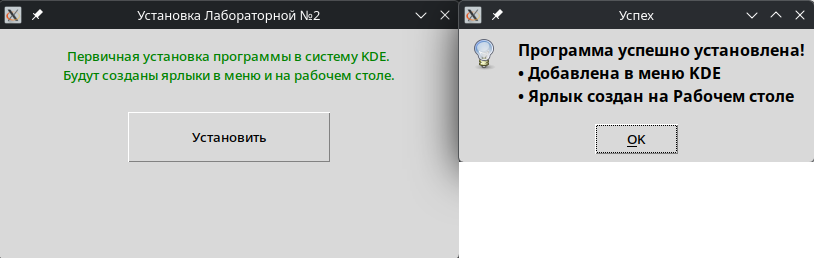
\includegraphics[width=0.88\textwidth,keepaspectratio]{img1.png}
    \caption{Диалоговое окно успешной установки программы в систему}
    \label{fig:installer}
\end{figure}


\begin{figure}[h!]
    \centering
    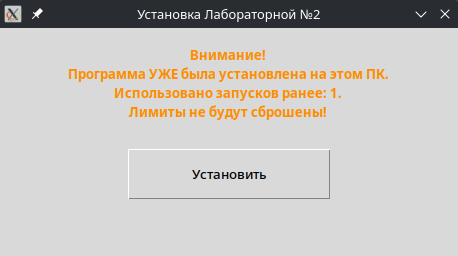
\includegraphics[width=0.6\textwidth,keepaspectratio]{img5.png}
    \caption{Диалоговое окно предупреждения о повторной установке программы с сохранением лимитов}
    \label{fig:previous_installer}
\end{figure}

\subsection{Эксплуатация программы}
Запуск приложения доступен как через иконку «Лабораторная 2 (Trial)» в главном меню приложений рабочего окружения или на Рабочем столе, так и из терминала:
\begin{lstlisting}[language=bash]
~/.local/share/lab2/main
# либо в среде разработки
python3 main.py
\end{lstlisting}

При открытии главного окна программы (Рисунок \ref{fig:main_window}) пользователь видит:
\begin{itemize}
    \item В верхней части отображается ранее сохраненное ФИО (если запись уже производилась) либо приглашение к вводу;
    \item В нижней части окна отображается статус триального периода: «Бесплатных запусков осталось: N»;
    \item Введите ФИО и нажмите кнопку «Сохранить». Данные запишутся на диск, а счетчик оставшихся попыток уменьшится.
\end{itemize}


\begin{figure}[h!]
    \centering
    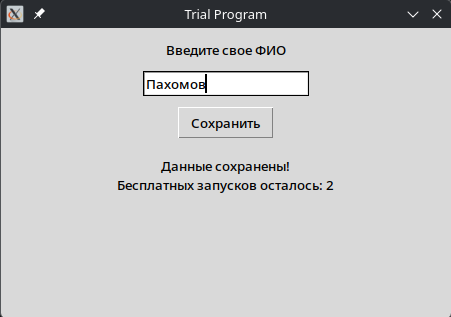
\includegraphics[width=0.6\textwidth,keepaspectratio]{img2.png}
    \caption{Главное окно программы с полем ввода ФИО и информацией о лимите запусков}
    \label{fig:main_window}
\end{figure}

\subsection{Действия при истечении ознакомительного периода}
После совершения 3 запусков либо по истечении 1 минуты с момента первого включения:
\begin{enumerate}
    \item Поля ввода блокируются;
    \item Отображается красный статус ошибки («Вы превысили лимит запусков программы» либо «Вы превысили лимит времени использования программы»);
    \item Предоставляется кликабельная гиперссылка для связи с разработчиком;
    \item Появляется красная кнопка «Удалить программу (Деинсталляция)».
\end{enumerate}

Интерфейс блокировки показан на Рисунке \ref{fig:blocked_window}.

\begin{figure}[h!]
    \centering
    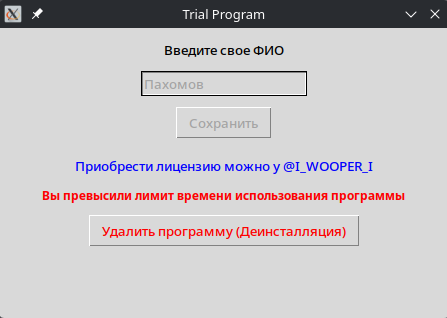
\includegraphics[width=0.6\textwidth,keepaspectratio]{img3.png}
    \caption{Главное окно программы в режиме блокировки после исчерпания лимитов}
    \label{fig:blocked_window}
\end{figure}

\subsection{Деинсталляция}
При нажатии на кнопку удаления или ручном запуске модуля \texttt{uninstaller.py}:
\begin{enumerate}
    \item Подтвердите согласие в диалоговом окне подтверждения;
    \item Программа удалит бинарные файлы и ярлыки, уведомив об успешном завершении операции.
\end{enumerate}

Интерфейс деинсталлятора показан на Рисунке \ref{fig:uninstaller}.

\begin{figure}[h!]
    \centering
    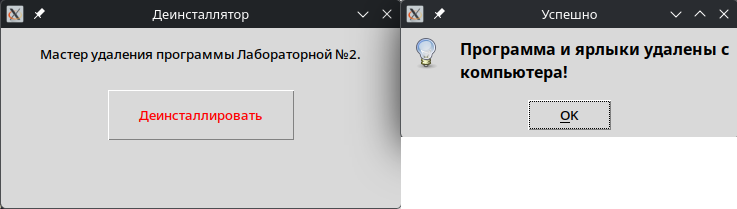
\includegraphics[width=0.7\textwidth,keepaspectratio]{img4.png}
    \caption{Диалоговое окно деинсталлятора с подтверждением удаления программы}
    \label{fig:uninstaller}
\end{figure}


% =========================================================================
% ЗАКЛЮЧЕНИЕ
% =========================================================================
\newpage
\begin{center}
    {\bfseries \MakeUppercase{Заключение}}
\end{center}
\addcontentsline{toc}{section}{ЗАКЛЮЧЕНИЕ}

В процессе выполнения лабораторной работы №2 был спроектирован, реализован и всесторонне протестирован программный комплекс защиты условно-бесплатного приложения (Trial-версии) от несанкционированного тиражирования и неправомерного продления пробного периода.

\textbf{Основные результаты работы}:
\begin{enumerate}
    \item Разработан графический инсталлятор (\texttt{installer.py}), интегрирующий приложение в рабочее окружение Linux/KDE через спецификации freedesktop/XDG и осуществляющий детектирование предыдущих установок продукта на целевой рабочей станции.
    \item Реализована основная программа (\texttt{main.py}) с графическим интерфейсом на базе Tkinter, обеспечивающая сбор, хранение и валидацию ФИО пользователя.
    \item Реализован комбинированный механизм защиты с параллельным контролем двух метрик: лимита на суммарное число запусков (Start-limited) и временного окна использования с момента первого старта (Time-limited).
    \item Разработан деинсталлятор (\texttt{uninstaller.py}), удаляющий исполняемые файлы и ярлыки рабочего стола, но сохраняющий системный скрытый артефакт в каталоге конфигураций, что исключает сброс лимитов при переустановке.
    \item Проведен анализ слабых мест реализованной архитектуры хранения лицензий и сформулированы практические рекомендации по повышению стойкости защиты от реверс-инжиниринга и локального взлома.
\end{enumerate}

% =========================================================================
% ПРИЛОЖЕНИЕ: ИСХОДНЫЙ КОД МОДУЛЕЙ СИСТЕМЫ
% =========================================================================
\newpage
\section*{ПРИЛОЖЕНИЕ. Листинги исходного кода}
\addcontentsline{toc}{section}{ПРИЛОЖЕНИЕ. ЛИСТИНГИ ИСХОДНОГО КОДА}

\subsection*{Листинг 1. Модуль инсталлятора (installer.py)}
\begin{lstlisting}[language=Python]
import os
import sys
import shutil
import subprocess
from tkinter import Tk, Label, Button, messagebox

def get_resource_path():
    """Получение пути к ресурсам при упаковке через PyInstaller"""
    if getattr(sys, 'frozen', False) and hasattr(sys, '_MEIPASS'):
        return sys._MEIPASS
    return os.path.dirname(os.path.abspath(__file__))

def get_desktop_dir():
    """Определение пути к каталогу Рабочего стола в соответствии со стандартами XDG"""
    try:
        res = subprocess.check_output(["xdg-user-dir", "DESKTOP"], text=True).strip()
        if os.path.exists(res):
            return res
    except Exception:
        pass
    
    for fallback in [os.path.expanduser("~/Desktop"), os.path.expanduser("~/Рабочий стол")]:
        if os.path.exists(fallback):
            return fallback
    return os.path.expanduser("~/Desktop")

BUNDLE_DIR = get_resource_path()
HOME = os.path.expanduser("~")

INSTALL_DIR = os.path.join(HOME, ".local", "share", "lab2")
APPS_DIR = os.path.join(HOME, ".local", "share", "applications")
DESKTOP_DIR = get_desktop_dir()

MENU_DESKTOP_FILE = os.path.join(APPS_DIR, "lab2.desktop")
DESKTOP_SHORTCUT_FILE = os.path.join(DESKTOP_DIR, "lab2.desktop")
CONF_FILE = os.path.join(HOME, ".config", "lab2", "lab2.txt")

def check_previous_install():
    """Проверка наличия следов предыдущей инсталляции и вычитка счетчика"""
    if os.path.exists(CONF_FILE):
        try:
            with open(CONF_FILE, "r") as f:
                lines = f.read().splitlines()
                if len(lines) >= 2 and int(lines[1]) > 0:
                    return True, int(lines[1])
        except Exception:
            pass
    return False, 0

def install():
    """Процедура развертывания исполняемых модулей и ярлыков в системе"""
    try:
        os.makedirs(INSTALL_DIR, exist_ok=True)
        os.makedirs(APPS_DIR, exist_ok=True)
        os.makedirs(DESKTOP_DIR, exist_ok=True)

        for filename in ["main", "uninstaller"]:
            src = os.path.join(BUNDLE_DIR, filename)
            if not os.path.exists(src):
                raise FileNotFoundError(f"Вшитый файл {filename} не найден!")

            dst = os.path.join(INSTALL_DIR, filename)
            shutil.copy2(src, dst)
            os.chmod(dst, 0o755)

        exec_path = os.path.join(INSTALL_DIR, "main")
        desktop_content = f"""[Desktop Entry]
Version=1.0
Type=Application
Name=Лабораторная 2 (Trial)
Comment=Программа с контролем запусков
Exec={exec_path}
Icon=system-lock-screen
Terminal=false
Categories=Utility;Application;
StartupNotify=true
"""
        # Создание пункта в меню приложений
        with open(MENU_DESKTOP_FILE, "w", encoding="utf-8") as f:
            f.write(desktop_content)
        os.chmod(MENU_DESKTOP_FILE, 0o755)

        # Создание ярлыка на Рабочем столе
        with open(DESKTOP_SHORTCUT_FILE, "w", encoding="utf-8") as f:
            f.write(desktop_content)
        os.chmod(DESKTOP_SHORTCUT_FILE, 0o755)

        # Установка доверенного атрибута запуска для среды KDE/GNOME
        try:
            subprocess.run(["gio", "set", DESKTOP_SHORTCUT_FILE, "metadata::trusted", "true"], stderr=subprocess.DEVNULL)
        except Exception:
            pass

        messagebox.showinfo(
            "Успех", 
            "Программа успешно установлена!\n"
            "• Добавлена в меню KDE\n"
            "• Ярлык создан на Рабочем столе"
        )
        root.destroy()
    except Exception as e:
        messagebox.showerror("Ошибка", f"Не удалось установить: {e}")

root = Tk()
root.title("Установка Лабораторной №2")
root.geometry("460x230")
root.resizable(False, False)

was_installed, launches = check_previous_install()

if was_installed:
    lbl_status = Label(
        root, 
        text=f"Внимание!\nПрограмма УЖЕ была установлена на этом ПК.\nИспользовано запусков ранее: {launches}.\nЛимиты не будут сброшены!", 
        fg="darkorange",
        font=("sans-serif", 10, "bold")
    )
else:
    lbl_status = Label(
        root, 
        text="Первичная установка программы в систему KDE.\nБудут созданы ярлыки в меню и на рабочем столе.", 
        fg="green"
    )

lbl_status.pack(pady=15)
btn_install = Button(root, text="Установить", width=22, height=2, command=install)
btn_install.pack(pady=10)

root.mainloop()
\end{lstlisting}

\newpage
\subsection*{Листинг 2. Основная рабочая программа (main.py)}
\begin{lstlisting}[language=Python]
import datetime
import os
import subprocess
from tkinter import Button, Entry, Label, Tk, messagebox
import webbrowser

HOME_PATH = os.path.expanduser("~/.config/lab2")
CONF_FILE = "lab2.txt"
CONF_PATH = f"{HOME_PATH}/{CONF_FILE}"

INSTALL_DIR = os.path.expanduser("~/.local/share/lab2")

# Конфигурация ограничений ознакомительного периода
MAX_LAUNCHES = 3
MAX_LAUNCHES_DELTA = datetime.timedelta(minutes=1)

def is_trial_expired(launches: int, first_launch: datetime.datetime) -> bool:
    """Проверка наступления условий блокировки по счетчику или времени"""
    now = datetime.datetime.now(tz=datetime.timezone.utc)
    return (launches >= MAX_LAUNCHES) or (now - MAX_LAUNCHES_DELTA > first_launch)

def run_uninstaller():
    """Вызов деинсталлятора при блокировке программы"""
    possible_paths = [
        os.path.join(INSTALL_DIR, "uninstaller"),
        os.path.join(INSTALL_DIR, "uninstaller.py"),
        os.path.join(os.path.dirname(os.path.abspath(__file__)), "uninstaller"),
        os.path.join(os.path.dirname(os.path.abspath(__file__)), "uninstaller.py")
    ]

    uninstaller_path = None
    for path in possible_paths:
        if os.path.exists(path):
            uninstaller_path = path
            break

    if uninstaller_path:
        if uninstaller_path.endswith(".py"):
            subprocess.Popen(["python3", uninstaller_path])
        else:
            subprocess.Popen([uninstaller_path])
        root.destroy()
    else:
        messagebox.showerror("Ошибка", "Деинсталлятор не найден в системе!")

def show_error():
    """Переключение графического интерфейса в режим блокировки"""
    global entry, label_error, label_info, btn_uninstall
    
    error_message = (
        "Вы превысили лимит запусков программы"
        if conf["launches"] >= MAX_LAUNCHES
        else "Вы превысили лимит времени использования программы"
    )
    
    label_error = Label(text=error_message, fg="red", font=("sans-serif", 9, "bold"))
    label_error.pack(pady=3)
    
    entry.config(state="disabled")
    button.config(state="disabled")
    
    label_info.config(
        text="Приобрести лицензию можно у @I_WOOPER_I",
        fg="blue",
        cursor="hand2"
    )
    label_info.bind("<Button-1>", lambda e: webbrowser.open("https://t.me/I_WOOPER_I"))

    btn_uninstall = Button(
        root, 
        text="Удалить программу (Деинсталляция)", 
        fg="red", 
        command=run_uninstaller
    )
    btn_uninstall.pack(pady=5)

def read_conf():
    """Считывание конфигурации и первичная инициализация при первом старте"""
    with open(CONF_PATH, "r") as f:
        conf = f.read().split("\n")
    
    now = datetime.datetime.now(tz=datetime.timezone.utc)
    if len(conf) >= 3 and len(conf[1]) > 0 and len(conf[2]) > 0:
        new_conf = {
            "name": conf[0],
            "launches": int(conf[1]),
            "first_launch": datetime.datetime.fromisoformat(conf[2])
        }
    else:
        new_conf = {
            "name": "",
            "launches": 0,
            "first_launch": now
        }
    return new_conf

def save_conf():
    """Инкремент счетчика и сохранение ФИО в файл"""
    global entry, conf, label_error, label_info

    if is_trial_expired(conf["launches"], conf["first_launch"]):
        show_error()
        return 
        
    conf["name"] = entry.get() or ""
    conf["launches"] = conf.get("launches", 0) + 1
        
    with open(CONF_PATH, "w") as f:
        f.write("\n".join(str(v) for v in conf.values()))

    label_info.config(
        text="Данные сохранены!\n" + f"Бесплатных запусков осталось: {MAX_LAUNCHES - conf['launches']}"
    )
    
    if is_trial_expired(conf["launches"], conf["first_launch"]):
        show_error()

if not os.path.exists(CONF_PATH):
    os.makedirs(HOME_PATH, exist_ok=True)
    with open(CONF_PATH, "w") as f:
        f.write("")
conf = read_conf()  

root = Tk()
root.title("Trial Program")
root.geometry("450x290")
root.resizable(False, False)

label_name = Label(
    text=f"Ваше ФИО: {conf['name']}\nИзменить:" if len(conf["name"]) > 0 else "Введите свое ФИО"
)
label_name.pack(pady=10)

entry = Entry()
entry.pack()

button = Button(text="Сохранить", command=save_conf)
button.pack(pady=10)

remaining = MAX_LAUNCHES - conf["launches"]
label_info = Label(
    text=f"Бесплатных запусков осталось: {remaining}" if not is_trial_expired(conf["launches"], conf["first_launch"]) else ""
)
label_info.pack(pady=5)

if is_trial_expired(conf["launches"], conf["first_launch"]):
    show_error()

root.mainloop()
\end{lstlisting}

\newpage
\subsection*{Листинг 3. Модуль деинсталляции (uninstaller.py)}
\begin{lstlisting}[language=Python]
import os
import shutil
import subprocess
from tkinter import Tk, Label, Button, messagebox

def get_desktop_dir():
    """Получение папки Desktop согласно стандарту XDG"""
    try:
        res = subprocess.check_output(["xdg-user-dir", "DESKTOP"], text=True).strip()
        if os.path.exists(res):
            return res
    except Exception:
        pass
    for fallback in [os.path.expanduser("~/Desktop"), os.path.expanduser("~/Рабочий стол")]:
        if os.path.exists(fallback):
            return fallback
    return os.path.expanduser("~/Desktop")

HOME = os.path.expanduser("~")
INSTALL_DIR = os.path.join(HOME, ".local", "share", "lab2")
APPS_DIR = os.path.join(HOME, ".local", "share", "applications")
DESKTOP_DIR = get_desktop_dir()

MENU_DESKTOP_FILE = os.path.join(APPS_DIR, "lab2.desktop")
DESKTOP_SHORTCUT_FILE = os.path.join(DESKTOP_DIR, "lab2.desktop")

def uninstall():
    """Удаление исполняемых компонентов без удаления конфигурации лицензии"""
    confirm = messagebox.askyesno("Удаление", "Вы действительно хотите удалить программу?")
    if not confirm:
        return

    try:
        # 1. Удаление пункта в меню приложений KDE
        if os.path.exists(MENU_DESKTOP_FILE):
            os.remove(MENU_DESKTOP_FILE)

        # 2. Удаление ярлыка с Рабочего стола
        if os.path.exists(DESKTOP_SHORTCUT_FILE):
            os.remove(DESKTOP_SHORTCUT_FILE)

        # 3. Полное удаление директории установленного бинарного ПО
        if os.path.exists(INSTALL_DIR):
            shutil.rmtree(INSTALL_DIR)

        # 4. Обновление баз данных и сброс кэша рабочего окружения KDE
        subprocess.run(["update-desktop-database", APPS_DIR], stderr=subprocess.DEVNULL, stdout=subprocess.DEVNULL)
        for cmd in ["kbuildsycoca6", "kbuildsycoca5"]:
            try:
                subprocess.run([cmd, "--noincremental"], stderr=subprocess.DEVNULL, stdout=subprocess.DEVNULL)
                break
            except FileNotFoundError:
                continue

        # Лицензионный маркер ~/.config/lab2/lab2.txt намеренно НЕ удаляется!

        messagebox.showinfo("Успешно", "Программа и ярлыки удалены с компьютера!")
        root.destroy()
    except Exception as e:
        messagebox.showerror("Ошибка", f"Ошибка при удалении: {e}")

root = Tk()
root.title("Деинсталлятор")
root.geometry("400x180")
root.resizable(False, False)

lbl = Label(root, text="Мастер удаления программы Лабораторной №2.", pady=15)
lbl.pack()

btn = Button(root, text="Деинсталлировать", fg="red", width=20, height=2, command=uninstall)
btn.pack(pady=10)

root.mainloop()
\end{lstlisting}

\end{document}